
\section{Introduction}
\label{sec:introduction}
%%% General intro

\IEEEPARstart{T}{he} constant research and the rapid evolution of machine learning (ML) techniques for sensor data analytics represent a promising landscape for Internet-of-Things (IoT) endpoint applications. CNN-based models represent the essential building blocks in 2D pattern recognition tasks. Sensor-based applications such as mechanical fault diagnosis\cite{li2019sensor,dong2018rolling}, structural health monitoring (SHM)\cite{nagayama2007structural}, human activity recognition (HAR) \cite{wang2019deep}, hazardous gas detection\cite{kim2017hazardous} have been powered by CNN-based models in industry and academia.

Due to the high computational demands of CNNs, dedicated hardware is typically required to accelerate execution. In terms of computational throughput, graphics processing units (GPUs) offer the highest performance. In terms of power efficiency, ASIC and FPGA solutions are well known to be more energy efficient (than GPUs) \cite{nurvitadhi2017can}. As a result, numerous commercial ASIC and FPGA accelerators have been proposed, targeting both high performance computing (HPC) for data-centers and embedded systems applications \cite{abdelouahab2018accelerating, guo2017angel}.

However, most of these CNN accelerators have been implemented to target mid- to high-range FPGAs to compute intensive CNN models such as AlexNet, VGG-16, ResNet-18. The power supply demands, physical dimensions, air cooling and heat sink requirements, and in some cases their elevated costs make these implementations inadequate or even impossible on resource-constrained low-power IoT devices.

In this article, we propose a design exploration framework for floating-point custom shallow CNN acceleration targeting low-power, inexpensive embedded FPGAs. This framework integrates TensorFlow (TF) Lite library with delegate interfaces between software runtime and the proposed hardware architecture to accelerate \emph{Conv2D} and \emph{DepthwiseConv2D} tensor operations. We design a tensor processor (TP) as a low-power hardware engine with customizable resource utilization. To accelerate floating-point computation, we adopt the hybrid custom floating-point and logarithmic dot-product approximation technique\cite{nevarez2021accelerating}, which exploits the intrinsic error-resilience of neural networks \cite{venkataramani2015approximate}. Further on, we propose a quantize aware training method to maintain and increase inference accuracy with low-precision custom floating-point formats.

\begin{figure}[t!]
	\centering
	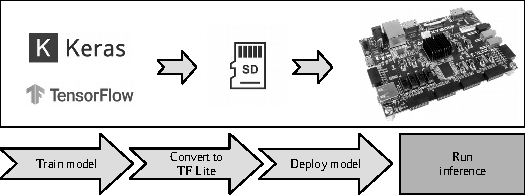
\includegraphics[width=0.5\textwidth]{../figures/workflow.pdf}
	\caption{The workflow of our approach on embedded FPGAs.}
	\label{fig:workflow}
\end{figure}

To operate the proposed system, the user would train a custom CNN model using TensorFlow or Keras, then this is converted into a TensorFlow Lite model, finally, the model is stored in a micro SD card along with the embedded software and configuration bitstream. (See \Fig{fig:workflow}.)

Our main contributions are as follows:
\begin{enumerate}
	\item We develop a hardware/software co-design framework targeting low-power, resource-limited embedded FPGAs for floating-point CNN acceleration. This is a scalable and parameterized architecture that allows design exploration integrated with TensorFlow Lite.
	\item We present a customizable tensor processor (TP) as a dedicated hardware accelerator. This TP computes \emph{Conv2D} and \emph{DepthwiseConv2D} tensor operations with hybrid custom floating-point formats and hybrid logarithmic approximation.
	\item we propose a quantize aware training method that maintains or increases inference accuracy with low-precision custom floating-point formats.
	\item We demonstrate the potential of the proposed architecture by addressing a design exploration with custom shallow CNN models using \emph{Conv2D} and \emph{DepthwiseConv2D} tensor operations. We evaluate compute performance and classification accuracy.
\end{enumerate}

The rest of the paper is organized as follows. Section~\ref{sec:related_work} covers the related work; Section~\ref{sec:background} introduces the background to \emph{Conv2D} and \emph{DepthwiseConv2D} tensor operations; Section~\ref{sec:system_design} describes the system design of the hardware/software architecture and the quantized aware training method; Section~\ref{sec:experimental_results} presents the experimental results thorough a design exploration flow; Section~\ref{sec:conclusions} concludes the paper.

To promote the research in this field, our entire work is made available to the public as an open-source project at (\emph{hidden for double blinded review}).